\subsection{Einleitung}
Die Website unseres Projekts dient als zentrales Bindeglied zwischen der technologischen Innovation unseres selbstfahrenden Golfcars und der globalen Gemeinschaft von Technikbegeisterten, Bildungseinrichtungen und potenziellen Nutzern. In diesem Abschnitt wird erläutert, wie die Planung und die Umsetzung der Website mit dem Ziel erfolgten, eine benutzerfreundliche, informative und interaktive Plattform zu schaffen. Wir stellen unsere Strategien für das Design, die Benutzerführung und die Inhaltsvermittlung vor und diskutieren, wie diese Elemente dazu beitragen, das Gesamtziel unseres Projekts zu unterstützen. Die Website ist nicht nur eine Darstellung unseres technischen Fortschritts, sondern auch ein Werkzeug, das es ermöglicht, die Fortschritte zu verfolgen, mit dem Team zu interagieren und das Projekt in seiner Entwicklung zu unterstützen.

\subsection{Zielgruppe}
\subsubsection{Hobbybastler}
Das Kernstück unseres Projekts, das selbstfahrende Miniatur-Golfcar, richtet sich an zwei Hauptzielgruppen: Hobbybastler und, in einer späteren Entwicklungsphase, Golfspieler. Hobbybastler stehen im Zentrum unserer Zielgruppe. Durch die Bereitstellung von Bauplänen, Bauteilen und Programmcode auf unserer Website schaffen wir eine Ressource, die es Enthusiasten ermöglicht, tief in die Materie der selbstfahrenden Autos einzutauchen. Unsere detaillierten Dokumentationen und Materialien dienen als Lerngrundlage und Inspirationsquelle für eigene Projekte. Diese Gruppe profitiert insbesondere von der Möglichkeit, die Theorie in die Praxis umzusetzen und durch unsere Anleitungen und Programme eigenständige Fortschritte zu erzielen.

\subsubsection{Golfspieler}
In einer zukünftigen Entwicklungsphase zielt unser Projekt darauf ab, auch Golfspieler anzusprechen. Die Vision ist es, ein Fahrzeug zu entwickeln, das auf Golfplätzen autonom verschossene Bälle lokalisieren und einsammeln kann. Dies würde nicht nur die Effizienz auf dem Golfplatz erhöhen, sondern auch ein neues Level an Technologieintegration in den Sport einführen. 

\subsubsection{Bildungseinrichtungen}
Als sekundäre Zielgruppe sehen wir Bildungseinheiten, wie Schulen und Universitäten, die unser Projekt als praktisches Lehrmittel nutzen könnten. Die Vielfalt der technischen Aspekte unseres selbstfahrenden Miniatur-Golfcars bietet eine ausgezeichnete Grundlage für interdisziplinäres Lernen und Experimentieren im Bereich der Robotik, Programmierung und Mechanik.

\subsection{Struktur der Website}

Die Website präsentiert sich mit einer klaren und nutzerzentrierten Struktur, die darauf ausgelegt ist, den Besuchern eine intuitive Bedienung und schnellen Zugriff auf die verschiedenen Sektionen zu ermöglichen.

\subsubsection{Navigationsleiste}
Die Website zeichnet sich durch eine innovative vertikale Navigationsleiste aus, die in der Mitte der Seite angeordnet ist. Bei einem Klick auf einen der Navigationspunkte (\textit{Home}, \textit{About}, \textit{Downloads}, \textit{Bauteile}, \textit{Live}, \textit{Teamspace}) öffnet sich dieser und präsentiert die jeweilige Seite, während die Leiste nach links versetzt wird. Ein erneuter Klick auf den bereits geöffneten Punkt lässt diesen wieder einziehen und zentriert die Navigationsleiste erneut.

\subsubsection{Interaktionselemente}
Die Website bietet verschiedene interaktive Elemente:
\begin{itemize}
    \item Ein \textbf{Live-View-Feature} im Adminbereich, das das Livebild der selbstfahrenden Autos anzeigt.
    \item Downloadbereiche, in denen Besucher alle relevanten Dokumente wie Baupläne, Diagramme und die Codebasis herunterladen können.
    \item Steuerelemente für das Auto, wie Buttons mit Pfeilen für die Richtungssteuerung und einen Start-Button für die automatische Suche.
    \item Ein Kontaktformular, um eine direkte Kommunikation mit dem Team zu ermöglichen.
\end{itemize}

\subsubsection{Usecase-Diagramm}
Ein Usecase-Diagramm wird ergänzt werden, um die Interaktionen der Nutzer mit den verschiedenen Funktionen der Website zu visualisieren. 

\newpage

\begin{figure}[h]
\centering
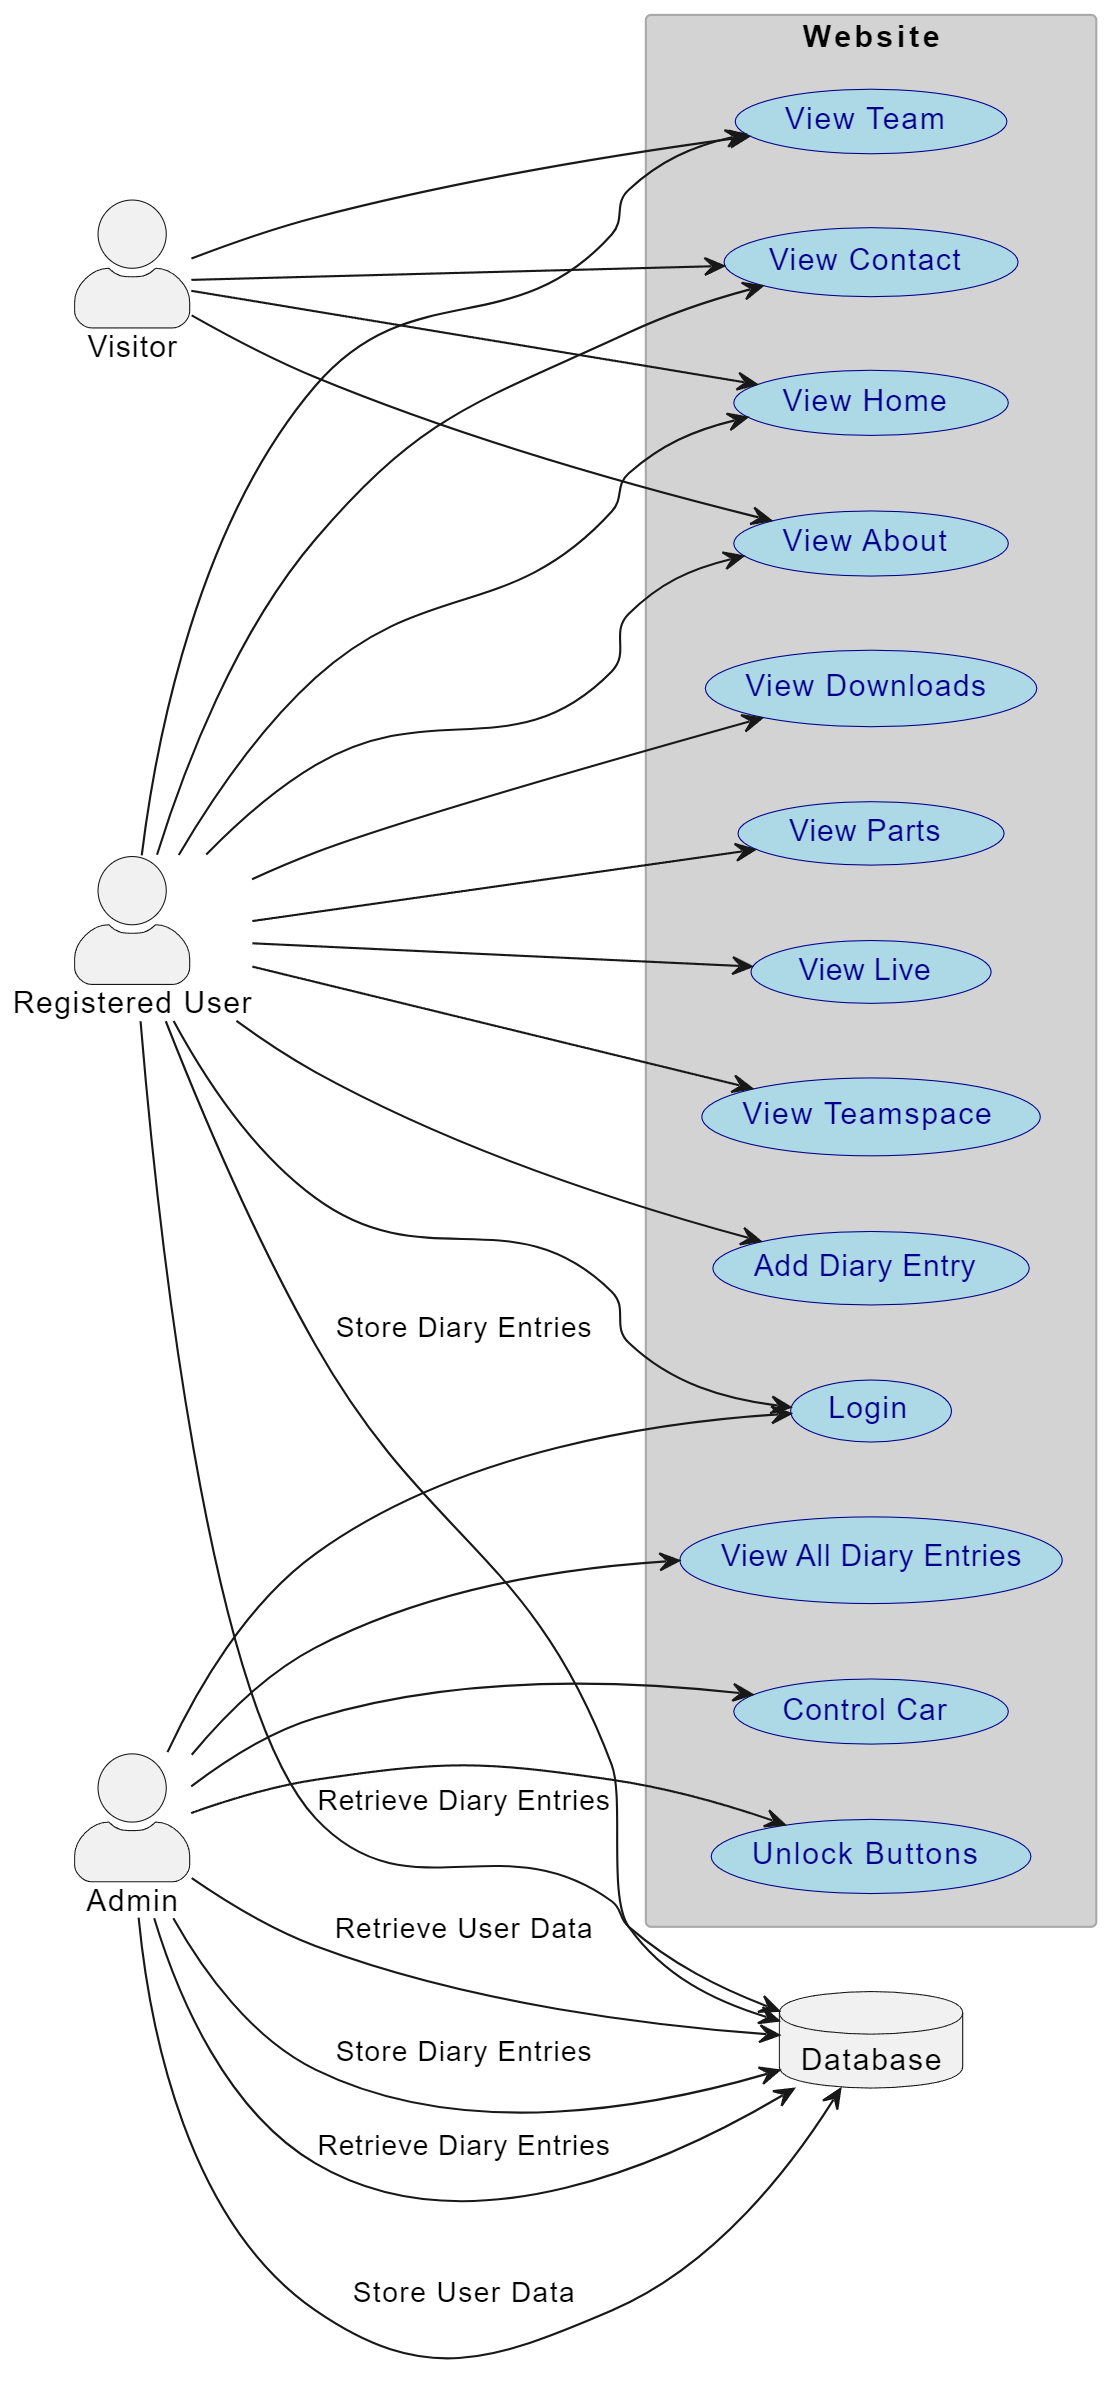
\includegraphics[width=0.52\textwidth]{Resources/diagram.png}
\caption{Usecase-Diagramm der Website-Interaktionen}
\end{figure}

\newpage

\subsection{Designraster und visuelle Gestaltung}

Das Design unserer Website ist von einem minimalistischen Ansatz geprägt, der sich auf das Wesentliche konzentriert und gleichzeitig ein einladendes und intuitives Benutzererlebnis bietet.

\subsubsection{Minimalistische Struktur}
Das Herzstück des Webdesigns ist die zentral positionierte, vertikale Menüleiste, die beim ersten Besuch der Website die alleinige Aufmerksamkeit auf sich zieht. Sie ist so konzipiert, dass sie das Bildschirmverhältnis im geschlossenen Zustand in drei gleich große Teile teilt, was eine harmonische Balance auf der Startseite schafft. Ein Klick auf eines der Menüelemente verlagert die Leiste nach links und öffnet den Inhalt des ausgewählten Menüpunkts auf der rechten Seite, im Verhältnis von etwa einem Drittel zu zwei Dritteln der Bildschirmbreite. Diese dynamische Bewegung verleiht der Seite eine lebendige Interaktivität und hält das Layout klar und fokussiert.

\subsubsection{Farbschema}
Die Hauptfarbe unserer Website ist ein sanftes Beige, repräsentiert durch das Farbquadrat nebenstehend, welches Ruhe und Wärme ausstrahlt und den minimalistischen Charakter unserer Website unterstreicht. Für einen starken Kontrast, der die Lesbarkeit insbesondere für Sehbehinderte erhöht, verwenden wir zusätzlich Schwarz in Texten und kritischen Interaktionselementen.

\noindent\raisebox{-0.7\height}{
\includegraphics[width=1cm]{Resources/color_sample.png}} \quad \raisebox{-0.7\height}{
\includegraphics[width=1cm]{Resources/color_sample_black.png}}

\subsubsection{Typografie und Lesbarkeit}
Die Typografie folgt dem Minimalismus der Seite, wobei klare, gut lesbare Schriftarten verwendet werden, die sowohl auf Bildschirmen als auch im Druck gut funktionieren. Große Schriftgrade und ausreichender Zeilenabstand gewährleisten eine hervorragende Lesbarkeit und Zugänglichkeit.

Als Hauptstandardschrift für Überschriften wurde \texttt{font-family: 'Cairo', sans-serif;} gewählt. Die Schriftart \textit{Cairo} ist bekannt für ihre moderne und klare Linienführung, die hilft, einen visuellen Eindruck von Ordnung und Sauberkeit zu vermitteln. Dies unterstützt den minimalistischen Ansatz der Website und fördert gleichzeitig eine starke visuelle Hierarchie, die es den Nutzern erleichtert, Inhalte schnell zu erfassen.

Ergänzend dazu wird \texttt{font-family: Arial, sans-serif;} für den Fließtext verwendet. \textit{Arial} ist eine extrem verbreitete und gut lesbare Schriftart, die aufgrund ihrer ausgezeichneten Lesbarkeit und ihrer unauffälligen Erscheinung auf einer Vielzahl von Geräten gut funktioniert. Dies trägt zur Konsistenz und Zugänglichkeit der Website bei, indem sichergestellt wird, dass Texte unter verschiedenen Betrachtungsbedingungen gut lesbar bleiben.

\subsubsection{Interaktionsdesign}
Das Interaktionsdesign ist so gestaltet, dass es sich nahtlos in die minimalistische Gestaltung einfügt. Die Übergänge sind glatt und die Benutzereingaben führen zu einer unmittelbaren und visuell ansprechenden Rückmeldung, was die Benutzererfahrung verbessert und ein Gefühl von Direktheit und Reaktionsfähigkeit vermittelt.

\subsubsection{Visuelle Hilfsmittel und Grafiken}
Die Verwendung von visuellen Hilfsmitteln und Grafiken ist sorgfältig dosiert. Sie ergänzen den Text, wo nötig, ohne die Benutzer von der Hauptbotschaft abzulenken. Die Grafiken sind so gestaltet, dass sie die Farbgebung aufgreifen und den Fokus auf die Interaktion verstärken.

\begin{figure}[h]
    \centering
    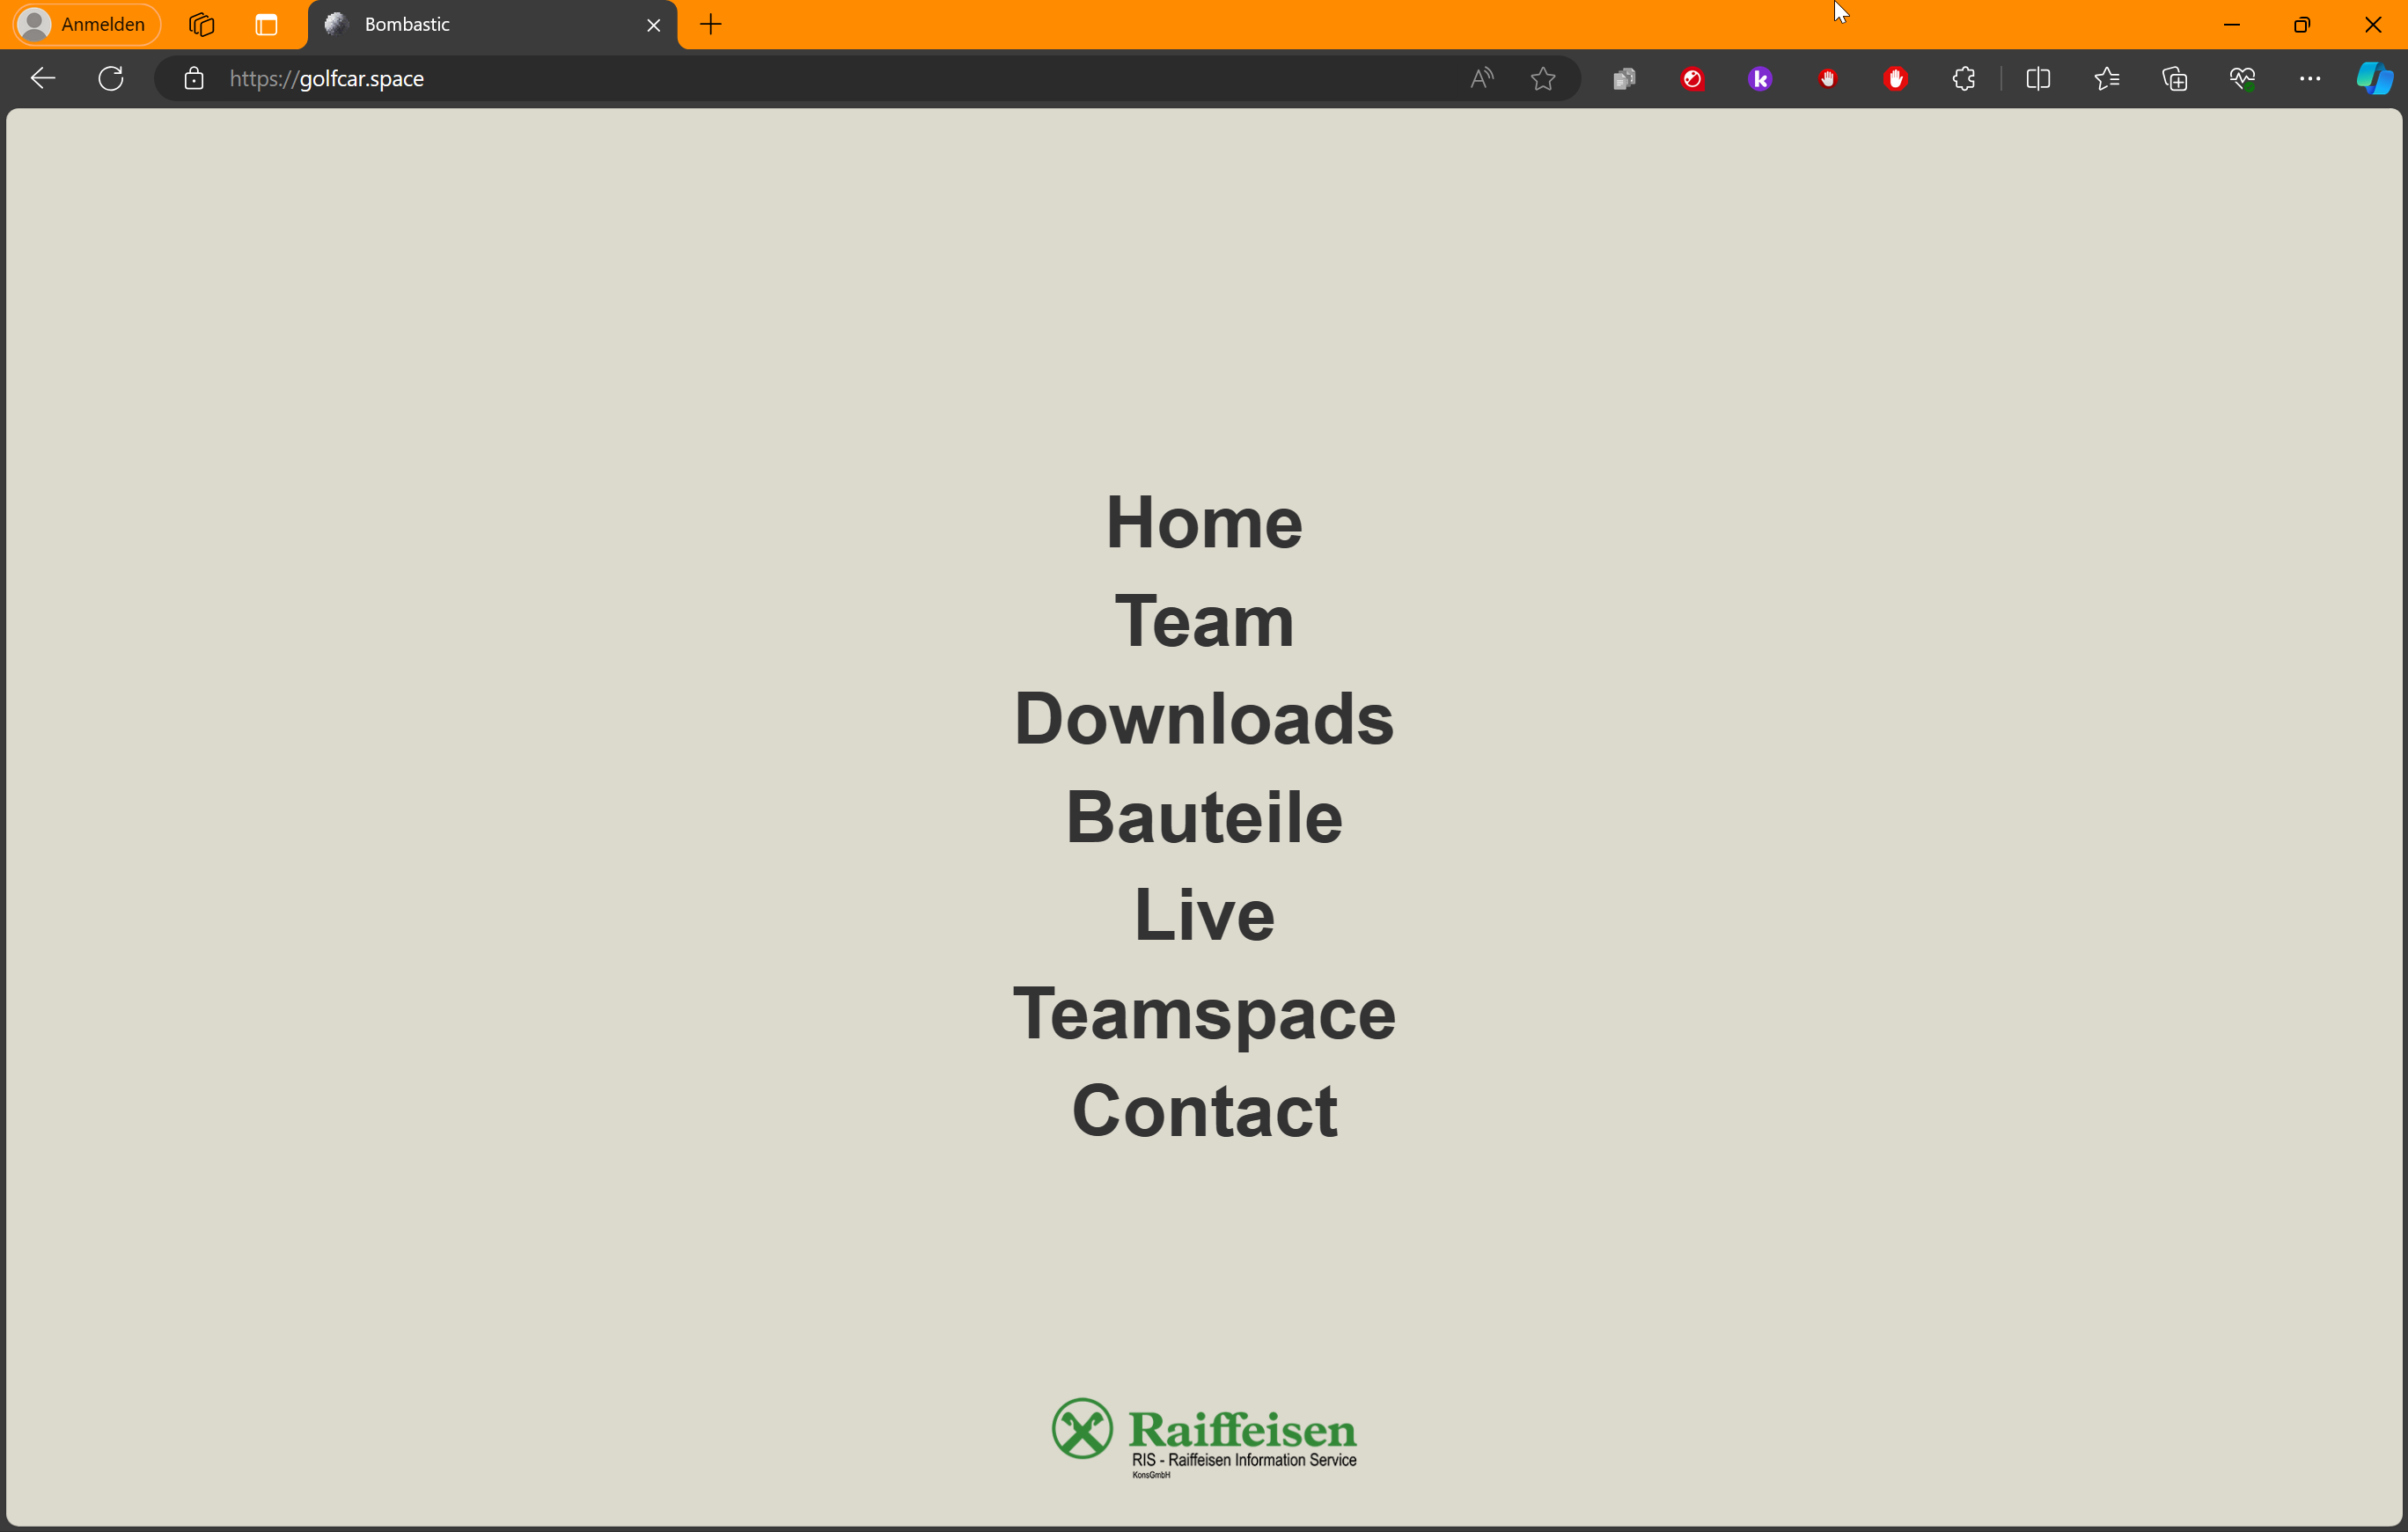
\includegraphics[width=\linewidth]{Resources/menu_screenshot.png}
    \caption{Screenshot des minimalistischen Menüs mit der Hauptfarbe im Hintergrund.}
    \end{figure}

%TODO: improve    
\subsection{Wirkung und Zielsetzung}

Die Gestaltung unserer Website zielt darauf ab, sowohl Benutzerfreundlichkeit als auch eine innovative Atmosphäre zu vermitteln. Unsere Vision ist es, eine futuristische Ästhetik zu schaffen, die sich in einer klaren, intuitiven Nutzerführung und einer sanften, ansprechenden Farbgestaltung widerspiegelt.

\subsubsection{Gesamteindruck und Emotionale Verbindung}
Beim Betreten der Website soll der Benutzer in eine Welt eintreten, die durch ein futuristisches Design geprägt ist, ohne dabei überladen zu wirken. Die zentrale Menüführung, unterstützt durch die weiche Farbgebung unseres Designs, lädt zum Entdecken und Verweilen ein, wobei die intuitive Benutzerführung das Engagement und die Interaktion fördert.

\subsubsection{Visionäre Kommunikation}
Die Vision des selbstfahrenden Golfcars wird durch minimalistische, aber ausdrucksstarke Grafiken kommuniziert, die die technologische Eleganz und die smarten Fähigkeiten des Autos hervorheben. Wir nutzen visuelle Metaphern, um die Innovation unseres Projekts zu betonen und die Stärken des Golfcars zu illustrieren.

\subsubsection{Call-to-Action}
Unser minimalistisches Menü fungiert als klarer Wegweiser für die Nutzeraktionen. Durch die einfache Auswahl der Menüpunkte wird der Benutzer ermutigt, die verschiedenen Aspekte unseres Projekts zu erkunden, von den technischen Details bis hin zur Live-Steuerung des Golfcars.

\subsubsection{Visuelles Konzept}
Für die bildliche Darstellung könnten wir abstrakte, technologieinspirierte Linienmuster verwenden, die Bewegung und Vernetzung symbolisieren. Grafiken von stilisierten Netzwerkdiagrammen oder schematischen Darstellungen des Golfcars könnten die futuristische und innovative Seite unseres Projekts betonen. Diese visuellen Elemente würden die Prinzipien des minimalistischen Designs aufgreifen und gleichzeitig die fortschrittliche Technik des selbstfahrenden Golfcars visualisieren.

%\begin{figure}[h]
%\centering
%\includegraphics[width=0.5\textwidth]{tech_graphic.png}
%\caption{Stilisierte Darstellung der Vernetzung und Technologie des Golfcars.}
%\end{figure}


\subsection{Ergonomie und Benutzerfreundlichkeit}

Die Ergonomie und Benutzerfreundlichkeit unserer Website sind zentrale Aspekte des Designs und der Entwicklung. Ziel ist es, allen Nutzern eine intuitive und angenehme Erfahrung zu bieten.

\subsubsection{Interaktionsdesign und Navigation}
Die Navigation auf unserer Website ist intuitiv gestaltet, um sicherzustellen, dass Benutzer schnell und effizient die gewünschten Informationen finden. Interaktive Elemente wie Buttons und Links sind klar erkennbar: Buttons sind deutlich als solche gestaltet, und Links sind traditionell blau und unterstrichen, um ihre Funktion offensichtlich zu machen. Hover-Effekte auf bestimmten Elementen bieten zusätzliche Informationen, was die Usability erhöht und Benutzern hilft, die Funktionalitäten besser zu verstehen.

\subsubsection{Feedback-Mechanismen}
Um eine interaktive und responsive Nutzererfahrung zu gewährleisten, implementiert die Website effektive Feedback-Mechanismen. Bei fehlerhaften Anmeldeversuchen, wie zum Beispiel durch die Eingabe eines falschen Benutzernamens oder Passworts, gibt der Browser sofort eine klare Fehlermeldung aus. Diese sofortige Rückmeldung hilft Benutzern, Korrekturen vorzunehmen und verbessert die allgemeine Benutzerinteraktion.

\subsubsection{Unterstützung für Sehbehinderte}
Auch die Bedürfnisse sehbehinderter Nutzer werden berücksichtigt. Überschriften und Zwischenüberschriften sind groß und gut lesbar gestaltet, mit hohem Kontrast, um die Lesbarkeit zu maximieren. Diese Designentscheidungen tragen dazu bei, die Zugänglichkeit unserer Website zu erhöhen.

\subsubsection{Optimierung der Ladezeiten}
Obwohl spezifische Maßnahmen zur Optimierung der Ladezeiten noch in Entwicklung sind, ist die Website bereits so konzipiert, dass sie effizient und schnell lädt. Zukünftige Updates werden weitere Verbesserungen in diesem Bereich bringen, um eine nahtlose Benutzererfahrung zu gewährleisten.

\subsubsection{Zukünftige Verbesserungen}
Wir planen, die Ergonomie und Benutzerfreundlichkeit kontinuierlich zu verbessern, indem wir Benutzerfeedback sammeln und analysieren. Die Umsetzung von Benutzervorschlägen wird uns helfen, die Website weiter zu optimieren und eine noch bessere Benutzererfahrung zu bieten.

\subsection{Grundlegende Überlegungen bei der Projektierung}

Bei der Entwicklung und dem Betrieb unserer Website für das selbstfahrende Miniatur-Golfcar-Projekt sind verschiedene Schlüsselfaktoren zu berücksichtigen, die für den Erfolg und die Reichweite unserer Online-Präsenz entscheidend sind.

\subsubsection{Werbung und Sichtbarkeit}

Um unser Projekt einem breiteren Publikum bekannt zu machen, planen wir den Einsatz von Google AdSense, gezielte Werbekampagnen auf Instagram sowie die Verteilung von Flyern in Schulen. Eine Kooperation mit Bildungseinrichtungen bietet sich an, um das Interesse von Lehrern und Schülern zu wecken und eine pädagogische Partnerschaft aufzubauen.

\subsubsection{Hosting und Zugänglichkeit}

In der Anfangsphase wird unsere Website auf einem Linux-Server unserer Schule gehostet, was den Zugriff zunächst auf das schulinterne Netzwerk beschränkt. Diese Vorgehensweise bietet einen kontrollierten Rahmen für die ersten Tests und die Weiterentwicklung der Website. In der Zukunft ist geplant, die Website auf einer öffentlichen Domain zu hosten, um das Projekt für alle Interessierten zugänglich zu machen.

\subsubsection{Qualitätssicherung und Versionierung}

Die Qualitätssicherung ist ein kontinuierlicher Prozess, der in Zusammenarbeit zwischen dem Projektleiter und den Webentwicklern durchgeführt wird. Wir nutzen Git für die Versionierung unserer Inhalte, um eine konsistente Weiterentwicklung und Fehlerbehebung zu gewährleisten. Im Impressum der Website wird die Aktualität der Inhalte durch Angabe des letzten Aktualisierungsdatums kommuniziert.

\subsubsection{Aktualisierung der Inhalte}

Neue Erkenntnisse, Fortschritte im Projekt und relevante Neuigkeiten werden regelmäßig auf der Website veröffentlicht, um unsere Besucher auf dem Laufenden zu halten. Diese Transparenz fördert das Vertrauen und die Einbindung der Community.

\subsubsection{Suchmaschinenoptimierung (SEO)}

Um die Auffindbarkeit unserer Website zu verbessern, setzen wir auf die Integration von Meta-Tags, die relevante Schlüsselwörter enthalten. Zusätzlich nutzen wir Google Analytics, um die Effektivität unserer Online-Präsenz zu bewerten und zu optimieren.

\paragraph{Meta-Tags und ihre Bedeutung}
Meta-Tags spielen eine entscheidende Rolle bei der Suchmaschinenoptimierung. Sie helfen Suchmaschinen, den Inhalt der Seiten besser zu verstehen und korrekt zu indizieren. Hier ein Beispiel der auf unserer Website verwendeten Meta-Tags:

\begin{lstlisting}
    <meta charset="UTF-8">
    <meta name="description" content="Schulprojekt Golfcar der Gruppe 6B-Engineering. Das Ziel: Ein selbstfahrendes Auto zu bauen, das einen Golfball automatisch in eine Box befoerdert">
    <meta name="keywords" content="Golfcar, Autonomous Car, ... , Educational Robotics, Open Source Hardware, IoT, Internet of Things, Maker Movement, Tech DIY, Electronic Components, Coding, Software Development, Hardware Programming">
    <meta name="robots" content="index, follow">
    <meta name="viewport" content="width=device-width, initial-scale=1.0">
    <meta name="author" content="6B Engineering">
    <!-- Open Graph Tags -->
    <meta property="og:title" content="6B-Engineering">
    <meta property="og:description" content="Schulprojekt Golfcar der Gruppe 6B-Engineering. Das Ziel: Ein selbstfahrendes Auto zu bauen, das einen Golfball automatisch in eine Box befoerdert">
\end{lstlisting}

\paragraph{Nutzung von Google Analytics}
Google Analytics hilft uns, die Besucherströme zu analysieren und die Wirkung unserer SEO-Maßnahmen zu verstehen. Diese Daten sind entscheidend für die kontinuierliche Optimierung unserer Inhalte und die Steigerung der Benutzerfreundlichkeit unserer Website.

\begin{figure}[h]
    \centering
    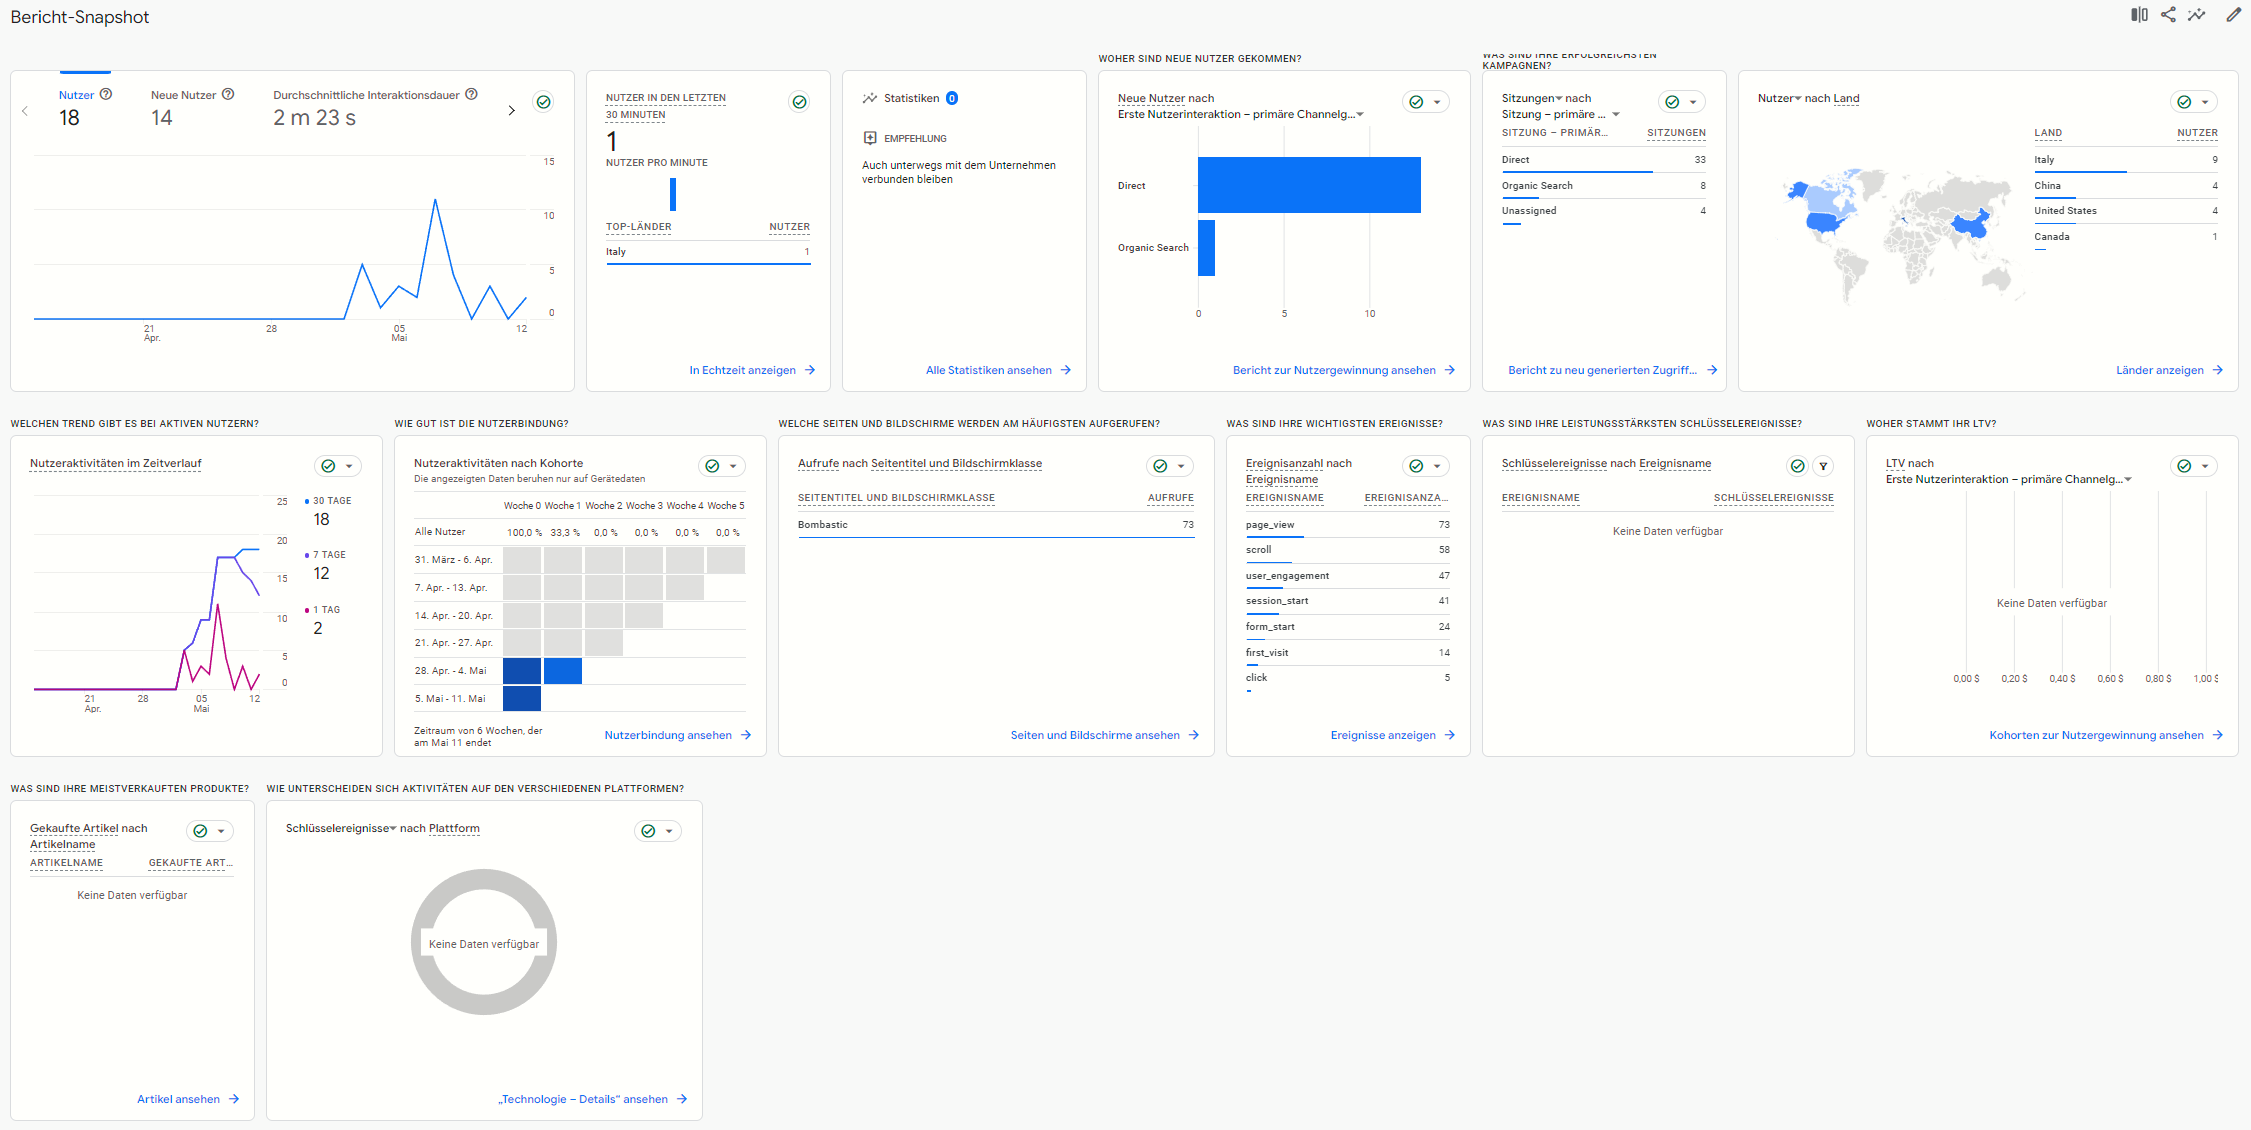
\includegraphics[width=\textwidth]{Resources/SEO_snapshot.png}
    \caption{Google Analytics Snapshot: Überblick über Nutzerinteraktionen und Engagement.}
\end{figure}

\newpage

\paragraph{Weitere Analyseergebnisse}
Die weiteren SEO-Analysebilder geben Einblick in verschiedene Nutzungsaspekte unserer Website:

\begin{figure}[h]
    \centering
    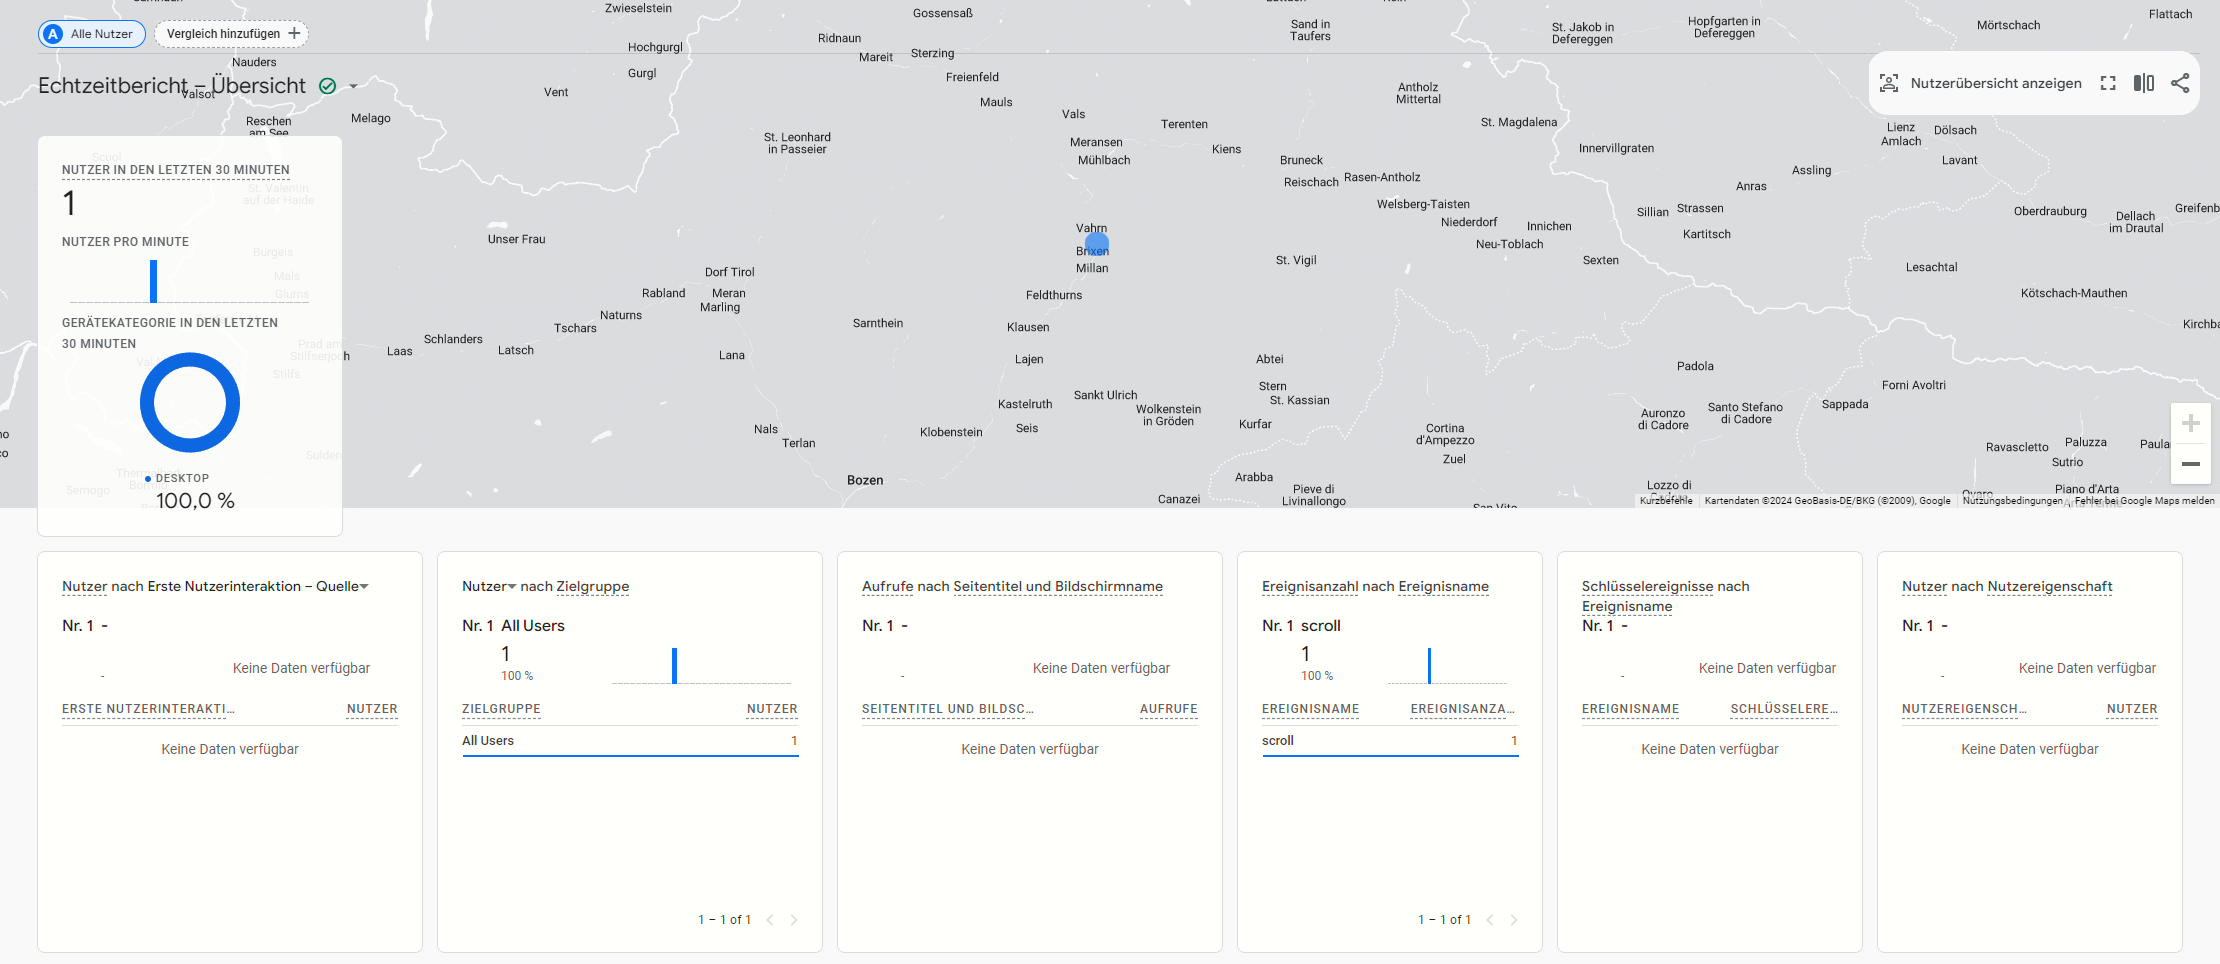
\includegraphics[width=\textwidth]{Resources/SEO_echtzeit.png}
    \caption{Echtzeit-Analyse: Aktive Nutzer und geographische Verteilung.}
\end{figure}

\begin{figure}[h]
    \centering
    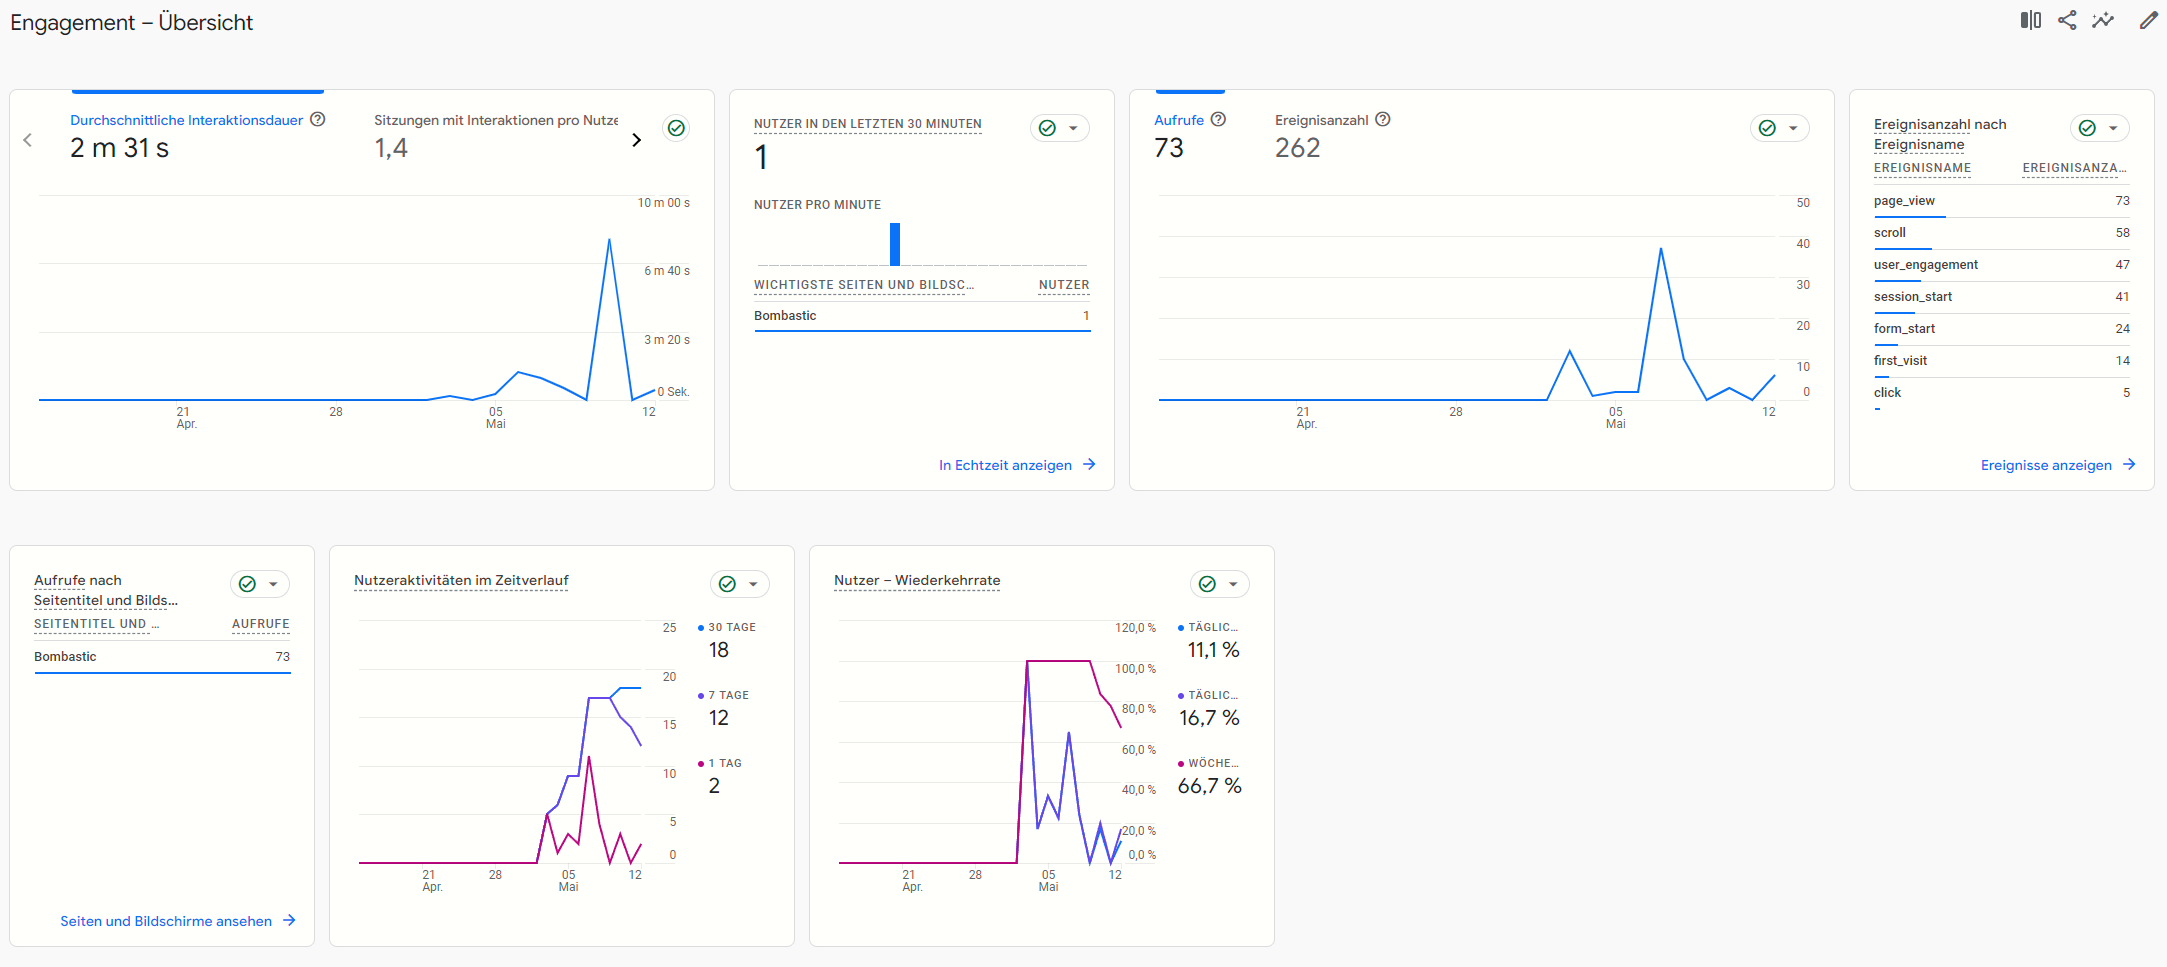
\includegraphics[width=\textwidth]{Resources/SEO_engagement.png}
    \caption{Nutzerengagement und Interaktionstiefe.}
\end{figure}

\newpage

\begin{figure}[h]
    \centering
    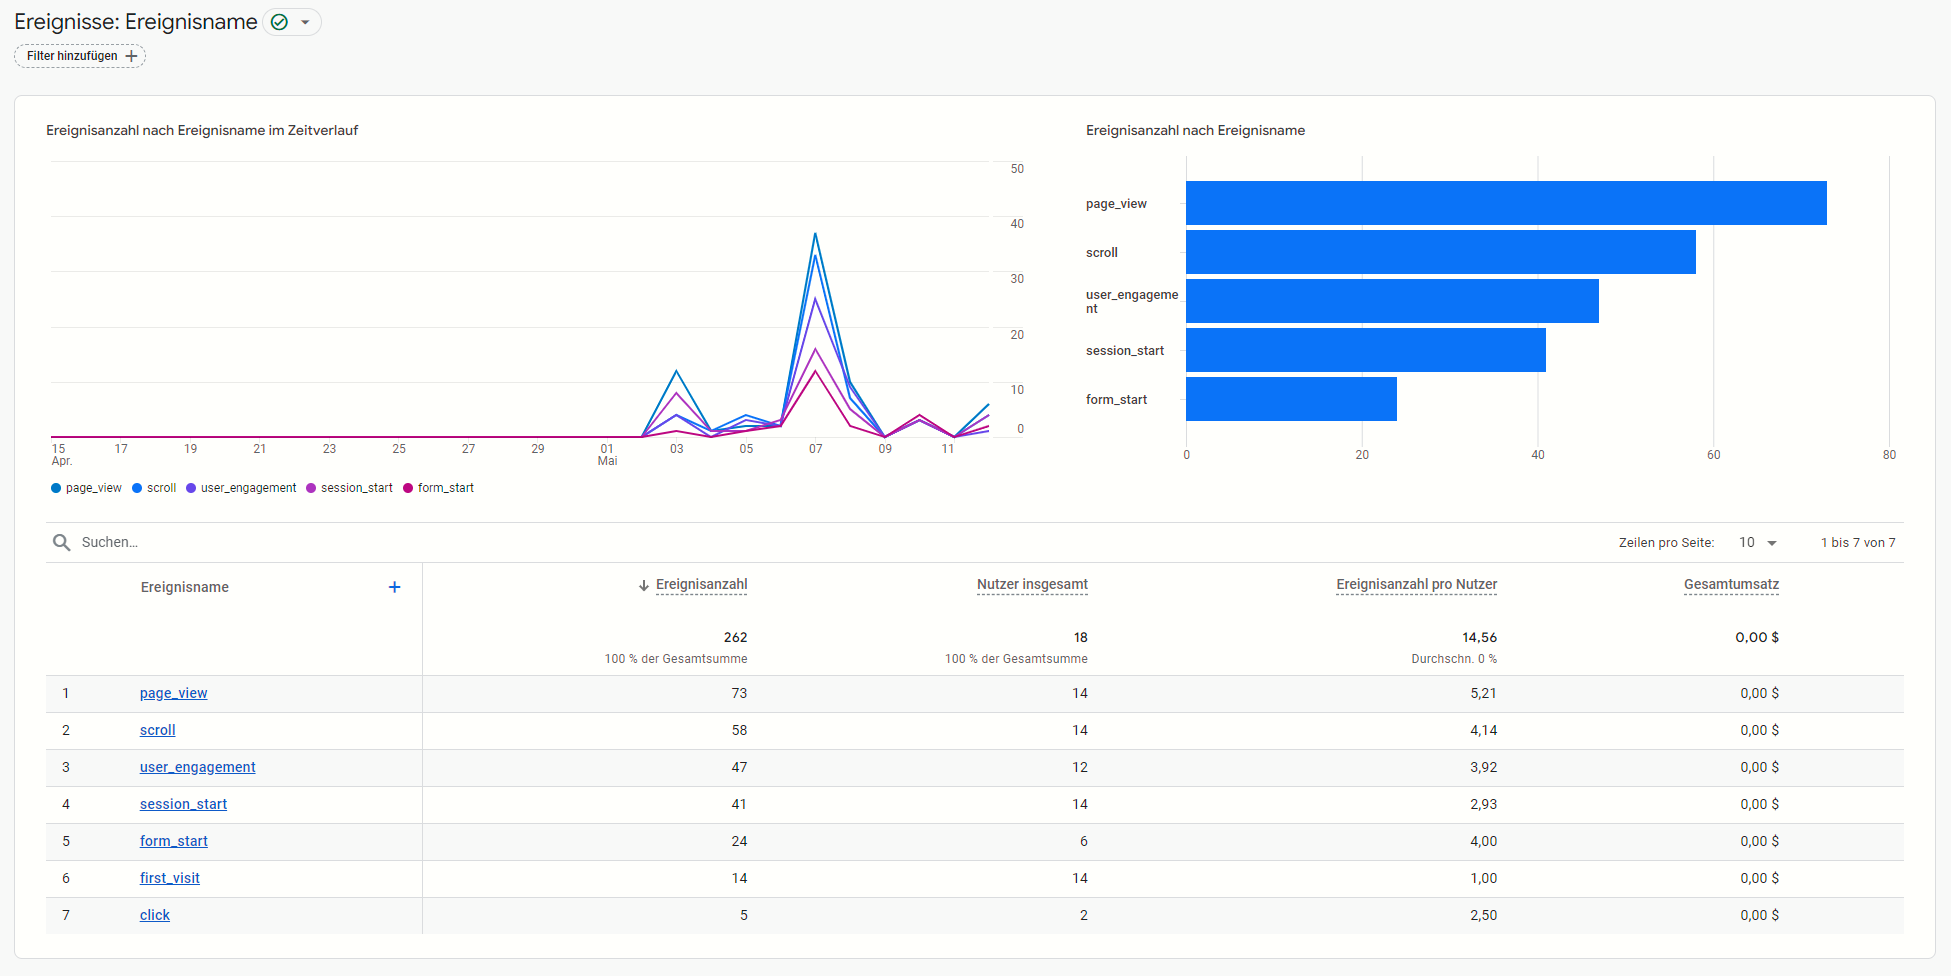
\includegraphics[width=\textwidth]{Resources/SEO_ergebnisse.png}
    \caption{Analyse der Ergebnisse und Nutzerfeedback.}
\end{figure}

\begin{figure}[h]
    \centering
    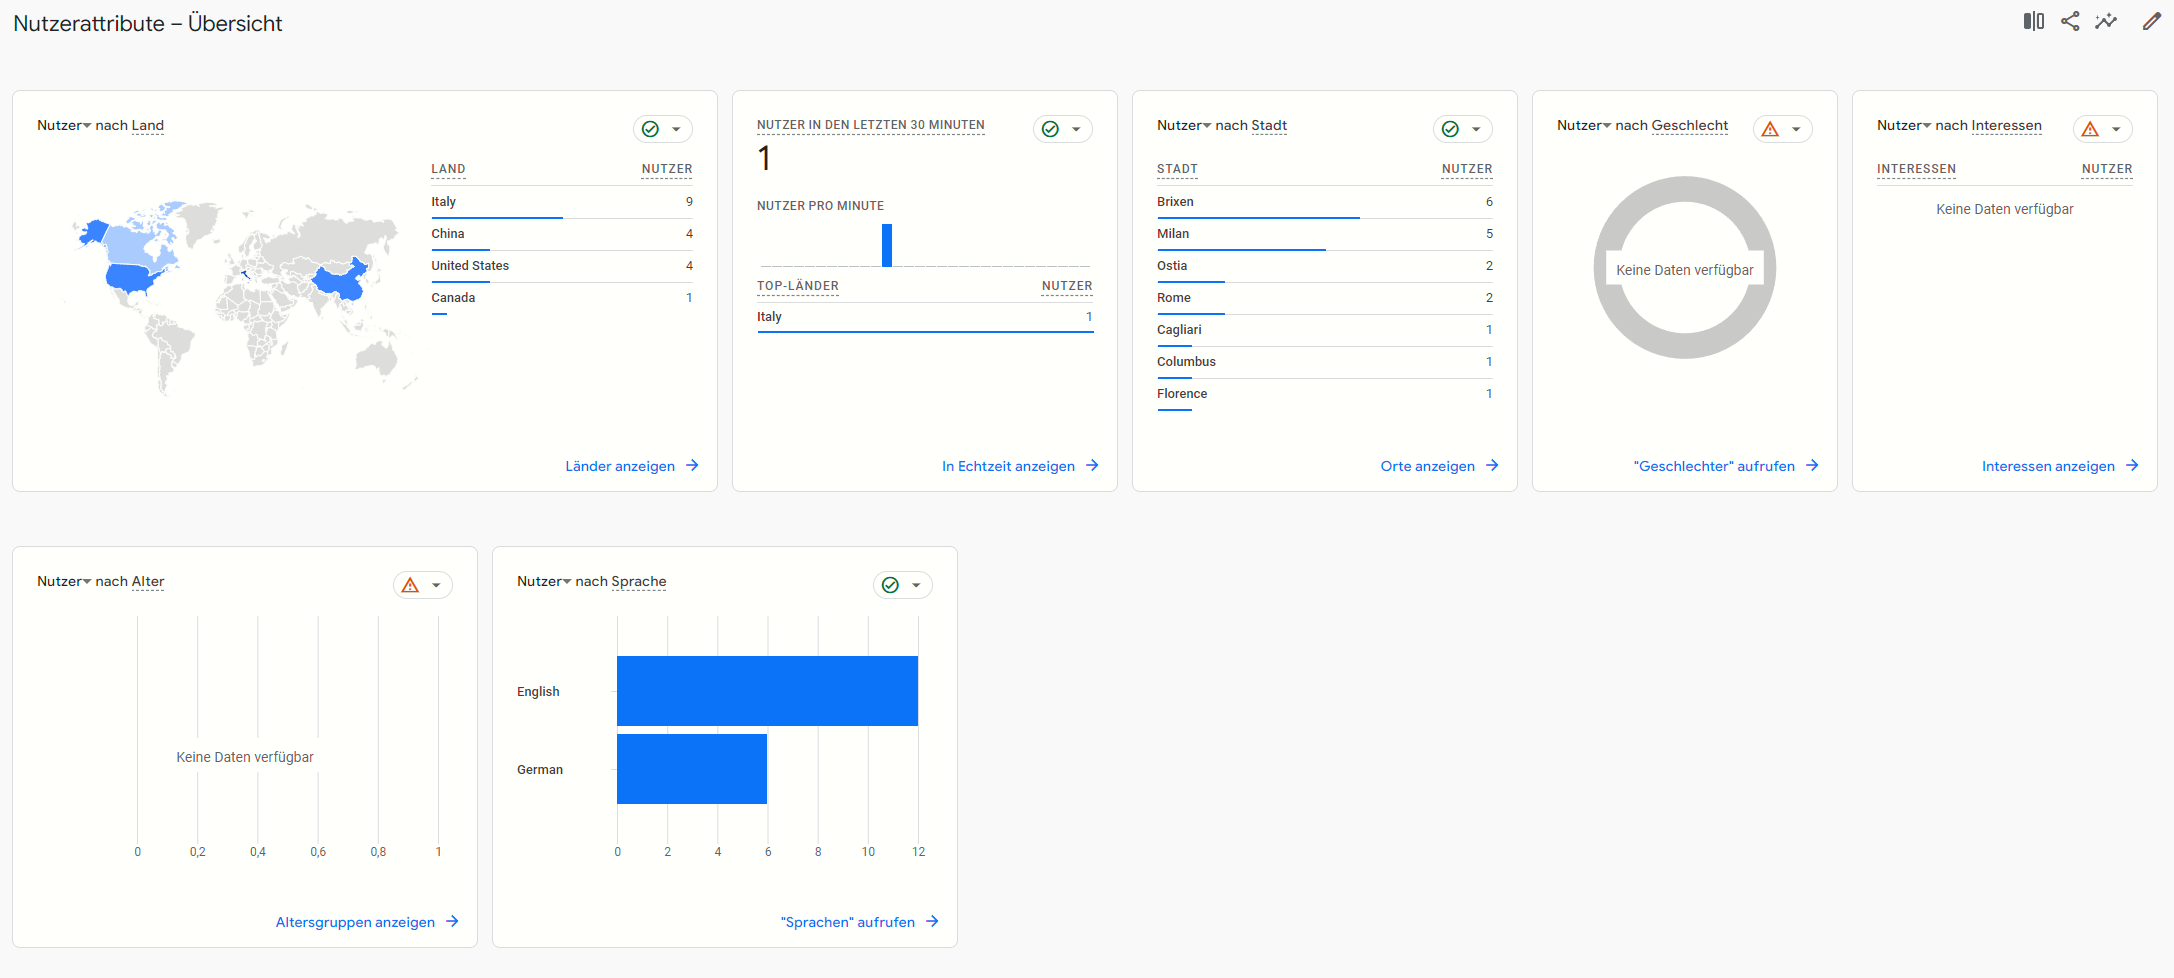
\includegraphics[width=\textwidth]{Resources/SEO_nutzerattribute.png}
    \caption{Detaillierte Attribute der Nutzer.}
\end{figure}

\newpage

\begin{figure}[h]
    \centering
    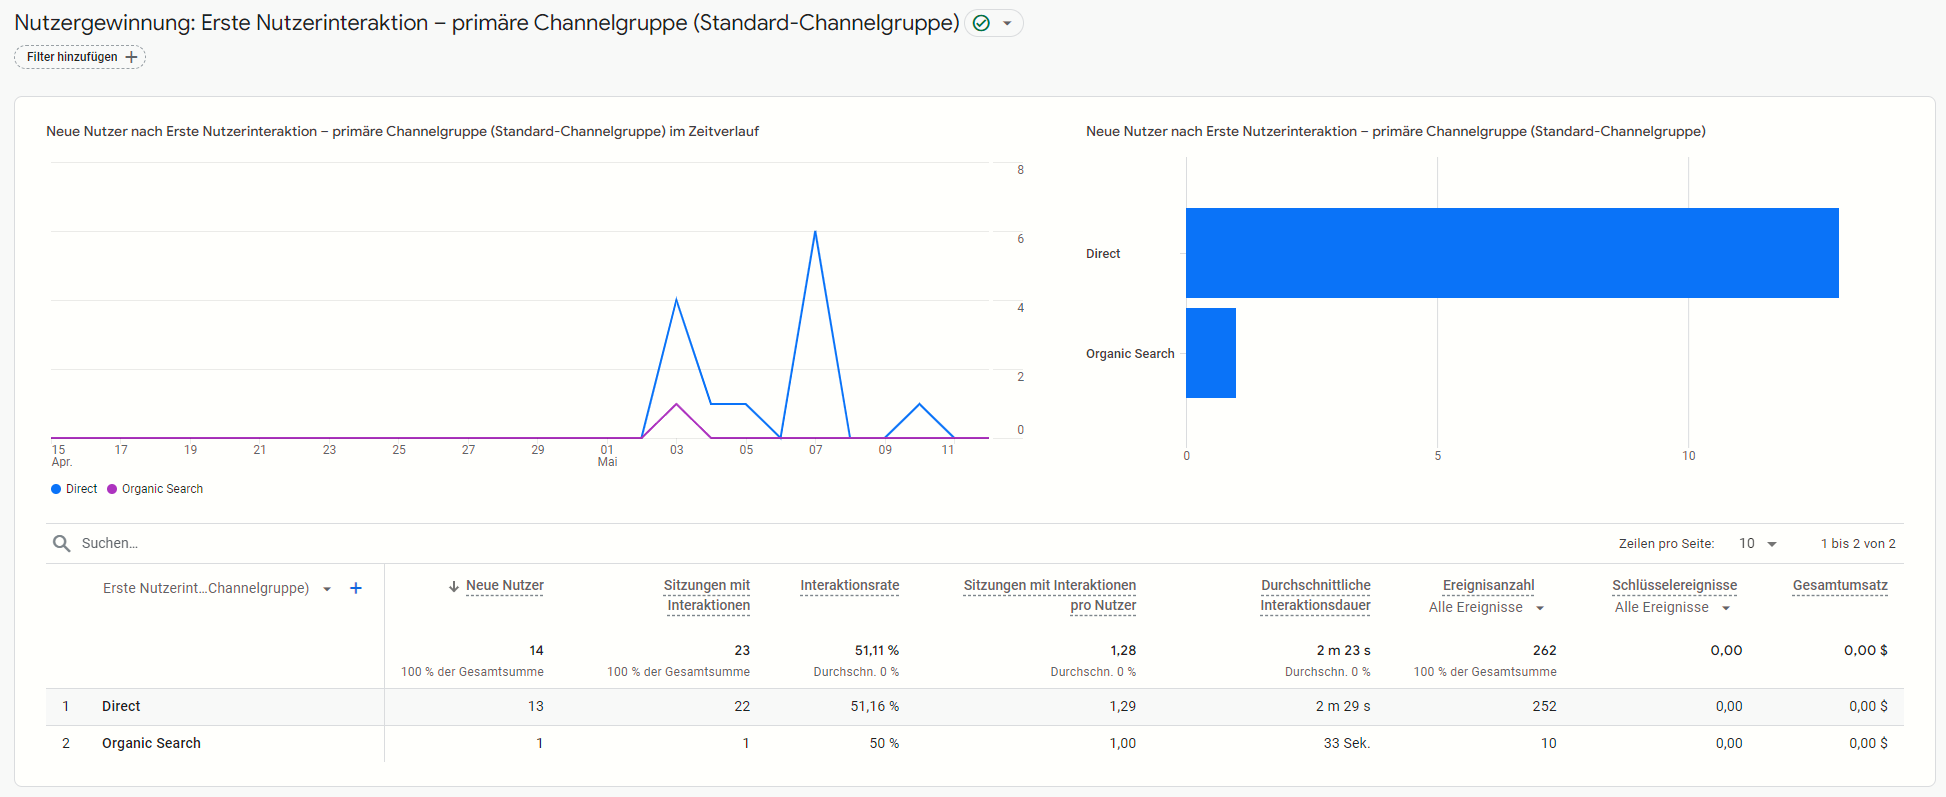
\includegraphics[width=\textwidth]{Resources/SEO_nutzergewinnung.png}
    \caption{Methoden der Nutzergewinnung und deren Effektivität.}
\end{figure}

\begin{figure}[h]
    \centering
    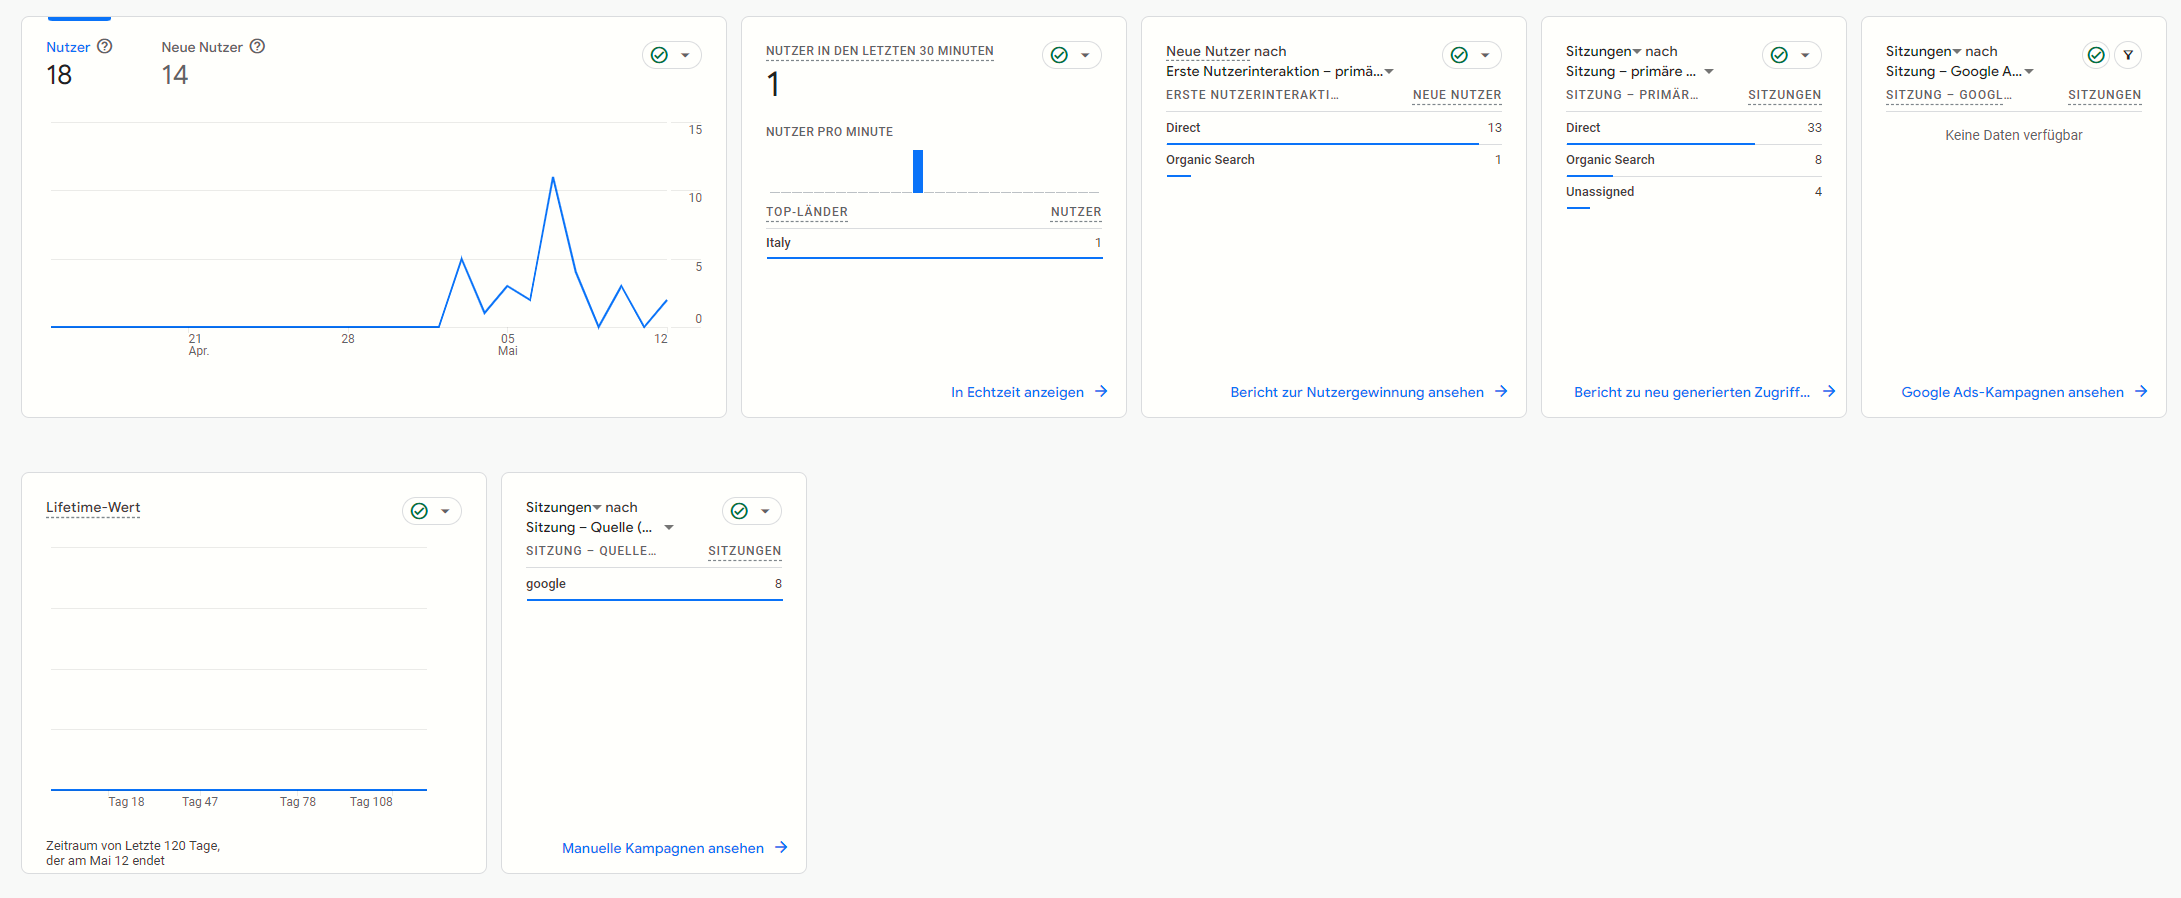
\includegraphics[width=\textwidth]{Resources/SEO_uebersicht.png}
    \caption{Umfassende Übersicht der SEO-Leistung und Nutzerdaten.}
\end{figure}

Diese umfangreichen Daten erlauben uns, fundierte Entscheidungen über zukünftige Anpassungen und Verbesserungen zu treffen, um die Besuchererfahrung weiter zu optimieren und unsere Website effektiv zu präsentieren.

\newpage

\subsection{Abschluss und Ausblick}

\subsubsection{Zusammenfassung der Ziele}
Die primären Ziele unserer Website waren die Präsentation des Teams, die Darstellung der Vision unseres selbstfahrenden Golfcar-Projekts sowie die Bereitstellung einer interaktiven Steuerung des Fahrzeugs über die Website. Diese Ziele wurden erfolgreich umgesetzt, was die Funktionalität und den innovativen Charakter unserer Plattform unterstreicht.

\subsubsection{Herausforderungen und Lösungen}
Während der Entwicklungsphase traten mehrere technische und organisatorische Herausforderungen auf:
\begin{itemize}
    \item \textbf{JSON-Dateien:} Anfängliche Schwierigkeiten im Umgang mit JSON-Dateien führten zu fehlerhaften Einträgen. Durch Implementierung zusätzlicher Kontrollabfragen und Formatierungschecks konnten diese Probleme behoben werden.
    \item \textbf{Edit Button:} Fehler durch die Verwendung von Anführungszeichen in Tagebucheinträgen wurden durch verbesserte Datenvalidierung gelöst.
    \item \textbf{Sicherheitsvorfall:} Nach einem Sicherheitsvorfall, verursacht durch einen Brute-Force-Angriff, haben wir die Sicherheitsmaßnahmen verschärft, indem wir Ports geändert, Anmeldedaten aktualisiert und automatische Sperrmechanismen für wiederholte Fehlanmeldungen (basierend auf der Software \textit{fail2ban}) implementiert haben.
\end{itemize}

\subsubsection{Feedback und Evaluation}
Das Feedback von Freunden und Klassenkameraden war entscheidend für die Optimierung der Website. Ihre Rückmeldungen zur Benutzerfreundlichkeit halfen uns, die Navigation und die allgemeine Benutzererfahrung zu verbessern.

\subsubsection{Langfristige Vision und zukünftige Entwicklungen}
Die langfristige Vision des Projekts ist die Veröffentlichung des gesamten Quellcodes auf GitHub nach der Projektvorstellung. Dies wird die Offenheit und Zugänglichkeit unserer Entwicklungsarbeit fördern und Interessierten ermöglichen, an der Weiterentwicklung teilzunehmen oder aus unseren Erfahrungen zu lernen. Aktuell sind keine weiteren spezifischen Ziele oder Meilensteine geplant.

\subsection{Aufruf zum Handeln}
Wir laden die Community ein, uns weiteres Feedback zu geben und sich an der Diskussion und Weiterentwicklung unseres Projekts zu beteiligen. Ihre Einsichten sind wertvoll für die fortlaufende Verbesserung und Anpassung unserer Website.

\subsection{Anhang}


\subsection{Literaturverzeichnis}
Das Literaturverzeichnis enthält alle referenzierten Quellen.
